\section{Measurement Procedure}

\subsection{Natural angular frequency}

\begin{enumerate}
\item Turn the Damping Selection knob to "0".
\item Rotate the balance wheel to the initial angular position $\theta_0 \approx
  150\degree$ and release it. Record the time of 10 periods. 
\item REpeat for four times and calculate the natural angular frequency
  $\omega_0$. 
\end{enumerate}

\subsection{Damping coefficient}

\begin{enumerate}    
\item Turn the Damping Selection knob to "2", and the selection should not be
  changed during this part. 
\item Rotate the balance wheel to the initial amplitude of approximately
  $150\degree$ and release it. Record the amplitude of each period and the time
  of 10 periods.  
\item The solution to the homogeneous equation of motion, with the corresponding
  initial conditions, is $\theta_{t}=\theta_0e^{-\beta t}cos(\omega_ft+\alpha)$.
  Hence $\theta_1=\theta_0e^{-\beta T}, \quad \theta_2=\theta_0e^{-\beta (2T)},
  \hdots, \theta_n=\theta_0e^{-\beta (nT)}$. The damping coefficient $\beta$ can
  then be calculated as 

\[ 
ln\frac{\theta_i}{\theta_j}=ln\frac{\theta_0e^{-\beta (iT)}}{\theta_0e^{-\beta
    (jT)}}=(j-i)\beta T. 
\]

\item The value of $T$ should be the average period, and
  $ln\frac{\theta_i}{\theta_{i+5}}$ should be obtained by the successive
  difference method as 

\[
\beta=\frac{1}{5T}ln\frac{\theta_i}{\theta_{i+5}}.
\]

\end{enumerate}

\begin{figure}[H]
\centering
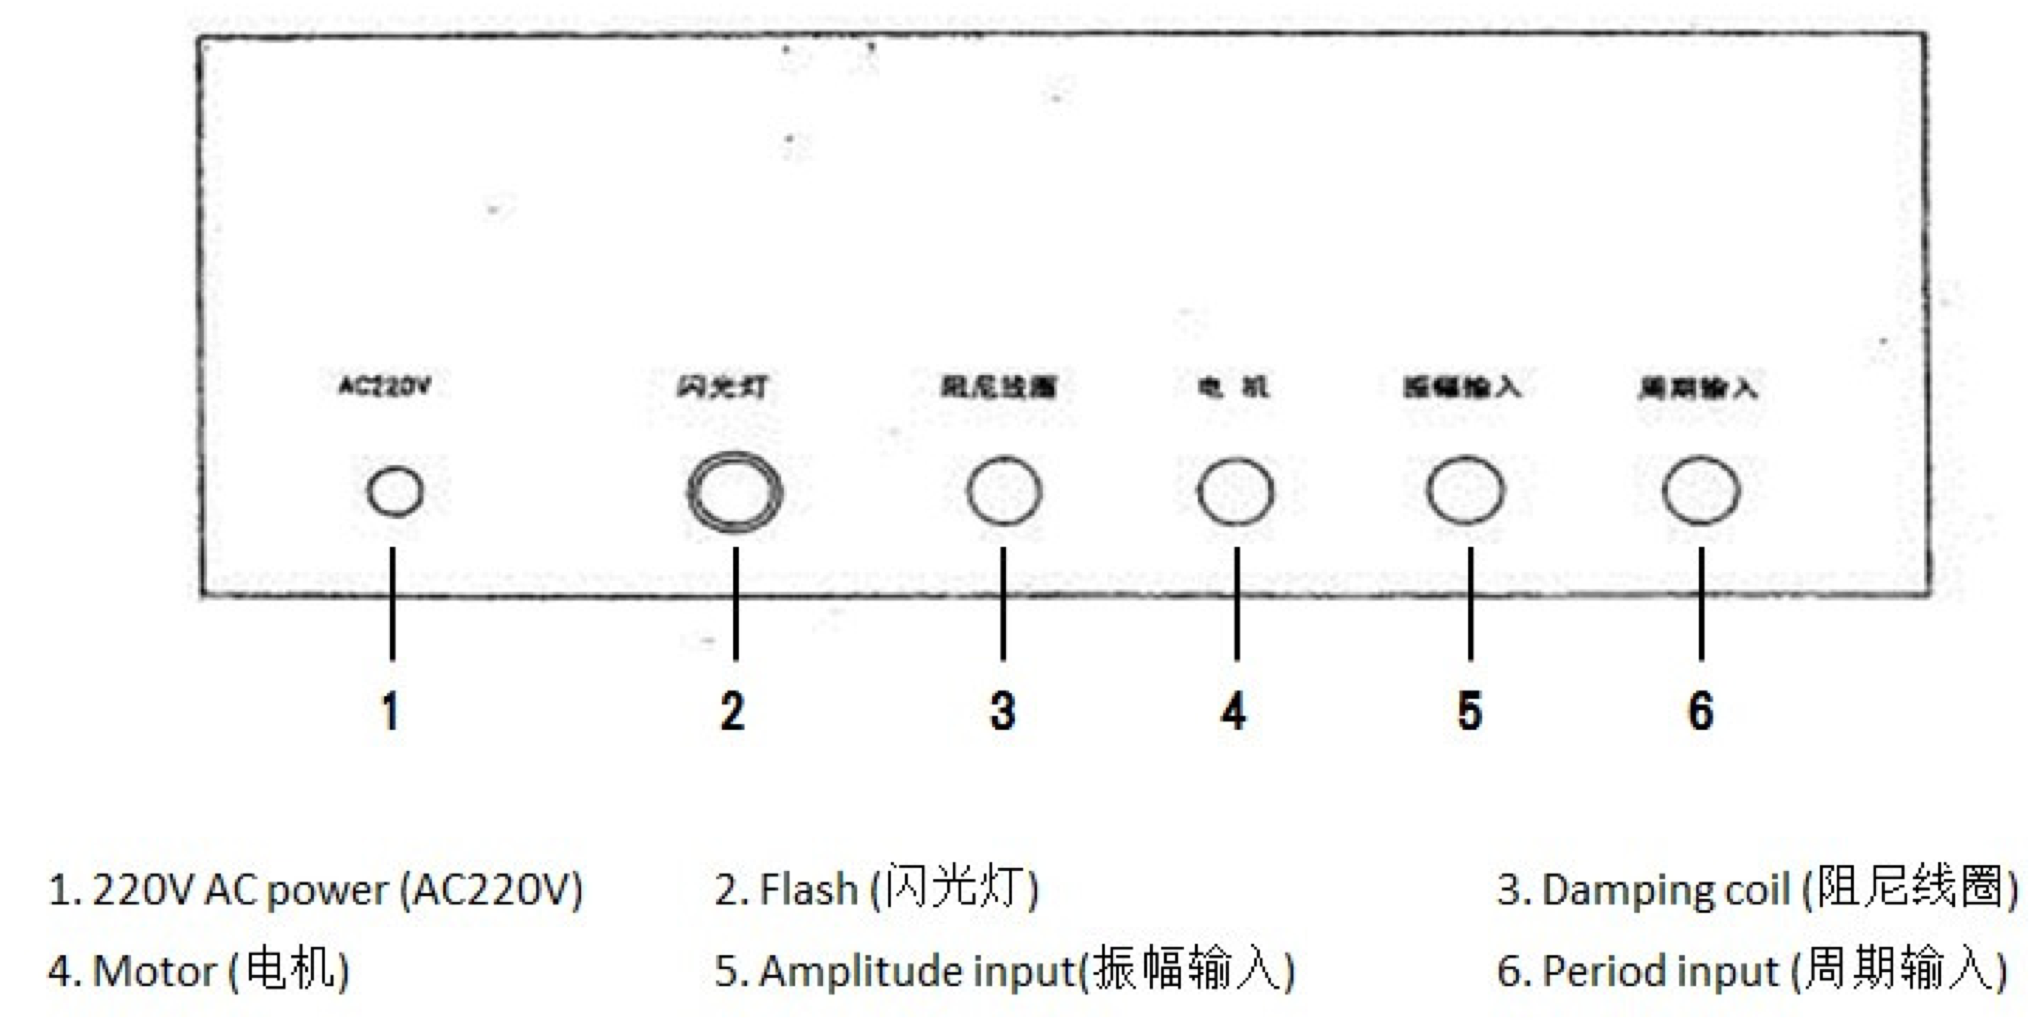
\includegraphics[width=0.7\textwidth]{fig/es4}
\caption{The rear panel of the control box}\label{real}
\end{figure}

\subsection{$\theta_{st}$ vs. $\omega$ and $\varphi$ vs. $\omega$
  Characteristics of forced oscillations} 

\begin{enumerate}
\item Keep the Damping Selection ar "2", and set the speed of the motor. Record
  the amplitude $\theta_{st}$, the period $T$, and the phase shift $\varphi$
  when the oscillation reaches a steady state. 
\item Repeat the steps above by changing the speed of the motor. It will result
  in a change of the phase shift $\varphi$ (referred to as $\Delta \varphi$).
  More data should be collected when $\varphi$ and $\theta_{st}$ change rapidly
  (e.g. near to the resonance point). At least 15 data should be collected for
  plotting.  
\item Choose Damping Selection "1" or "3". Repeat the above steps.
\item Plot the $\theta_{st} (\omega)$ characteristics, with $\omega/\omega_0$ on
  the horizontal axis and $\theta_{st}$ on the vertical axis. Two sets of data
  should be plotted on the same graph. 
Plot the $\varphi (\omega)$ characteristics, with $\omega/\omega_0$ on the
horizontal axis and $\varphi$ on the vertical axis. Two sets of data should be
plotted on the same graph. 
\end{enumerate}


